\section{Validación y comparación con la referencia real}
\label{sec:validacion}

\subsection{Qué se compara}
La condición nominal (demanda 1.00, \NReps{} réplicas) se compara con las cuatro métricas
generales de espera de NHAMCS 2022 derivadas de \texttt{WAITTIME}, con las mismas unidades:
espera media, mediana y percentil 90 (minutos) y proporción de pacientes con espera mayor a
60 minutos. \texttt{WAITTIME} no se usó para ajustar parámetros ni para seleccionar la
candidata, de modo que es una referencia independiente. El error de las tres métricas con
unidad de tiempo se resume con el error absoluto medio (MAE); la proporción se mantiene
aparte para no mezclar unidades.

\begin{table}[ht]
\centering\small
\caption{Referencia real, simulación base y simulación candidata, con las mismas métricas y
unidades. La referencia usa $n=\RefN$ visitas con \texttt{WAITTIME} válido (estimación
ponderada; los cuantiles no tienen error estándar). Simulación: media de \NReps{} réplicas.}
\label{tab:validacion}
\fittable{generated/tab_validation.tex}
\end{table}

\begin{figure}[ht]
\centering
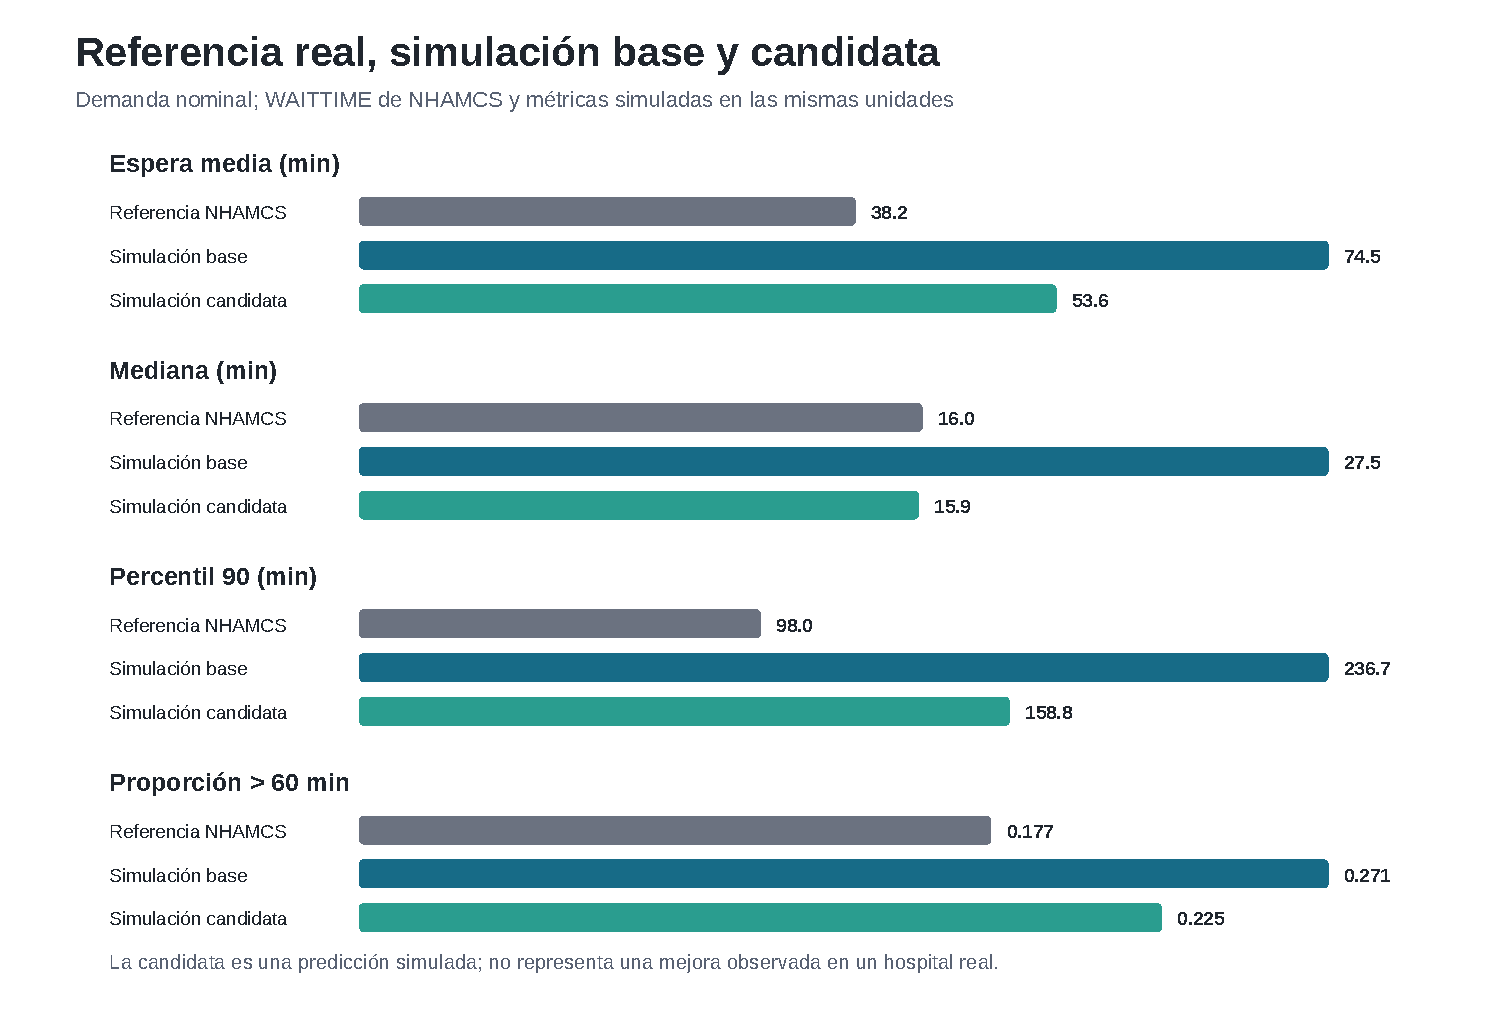
\includegraphics[width=0.92\linewidth]{figures/validation_comparison.pdf}
\caption{Comparación de la referencia NHAMCS 2022 con la simulación base y la candidata
(figura generada en \texttt{evidence/final/figures/}).}
\label{fig:validacion}
\end{figure}

\subsection{Interpretación}
\begin{itemize}
  \item El modelo base \textbf{sobreestima las cuatro métricas}: espera media de \WaitBaseNom{}
  frente a \RefMeanWait{} min (IC 95\,\% de la referencia [\RefMeanCILow, \RefMeanCIHigh]),
  y percentil 90 de \NomBasePninety{} frente a \RefPninetyWait{} min. Su MAE en minutos es
  \MaeBase{}; en la proporción, \MaePropBase{}.
  \item La candidata queda más cerca (MAE de \MaeCand{} min; \MaePropCand{} en la
  proporción). Su mediana (\NomCandMedian{} min) casi coincide con la referencia
  (\RefMedianWait{} min), pero el percentil 90 candidato sigue \PninetyCandErr{} min por
  encima de NHAMCS: el modelo reproduce peor la cola larga.
  \item Que la candidata se aproxime a la referencia \emph{no convierte la intervención en
  validada}: el algoritmo minimizó la espera simulada, no se ajustó a \texttt{WAITTIME}, y la
  referencia es el desempeño observado de departamentos heterogéneos, no el efecto de un
  cambio de horario.
\end{itemize}

\subsection{Límites de la comparación}
\texttt{WAITTIME} mide la espera hasta el primer contacto con médico, APRN o PA, mientras el
modelo mide la espera hasta que un equipo inicia la atención; las poblaciones también
difieren (promedio nacional de muchos DE frente a un DE sintético de volumen mediano). La
correspondencia del modelo es, por tanto, parcial. La discrepancia en la cola larga puede
deberse a un servicio supuesto demasiado largo, a la falta de variabilidad del proceso real
o a la diferencia de métrica; este informe no permite distinguir entre estas explicaciones.
